\documentclass[twoside,10pt]{article}
\usepackage{shlists}
\usepackage[applemac]{inputenc}
\usepackage[spanish]{babel}
\usepackage[T1]{fontenc}


\usepackage{multicol}
\usepackage{picinpar}

\usepackage{url}
\newcommand{\surl}[1]{{\small\url{#1}}}

\newcounter{vol}
\newcounter{num}
\newcounter{anyo}
\setcounter{vol}{9}
\setcounter{num}{2}
\setcounter{anyo}{2016}
\newcommand{\mes}{Mayo}
\usepackage{revisionNLcol}


\title{\ \\ Docencia 2.0\\ \large Juan Juli\'{a}n Merelo, Fernando Tricas}
\author{\LARGE Dise�ando un proyecto}

\date{}

\AutTit{Docencia 2.0}

\begin{document}
\addtocounter{page}{2}

\maketitle
\vspace*{-5ex}

\begin{multicols}{2}

Uno de los problemas a los que se enfrentan muchos alumnos, o
profesores, cuando tratan de proponer nuevos proyectos para una
asignatura o TFG (de los que hablamos, por cierto, no hace tanto en
esta columna:
\url{http://www.aenui.net/ojs/index.php?journal=revision&page=article&op=view&path[]=238&path[]=381})
es encontrar un tema que sea atractivo para el estudiante, que est� dentro
de la �rbita de los conocimientos de tutor y estudiante, y que tambi�n
lo acerque, dentro de lo posible, al mundo real. 

El cumplimiento de ese conjunto de restricciones hace que el campo
posible se reduzca mucho: extensiones de proyectos anteriores,
proyectos en los que el alumno est� trabajando si es que est�
relacionado con una empresa, o peque�os proyectos relacionados con la
investigaci�n del tutor. Sin embargo, no siempre se pueden cumplir
todas las restricciones y en ocasiones el requisito que se suele caer
de ese panel es el de acercarse al mundo real. Lo que es una pena,
porque como ya dijimos en la columna anterior, proyectos realizados,
siempre que se liberen, acaban formando parte de un portafolio que
ser� la carta de presentaci�n del estudiante ya graduado al mundo de
la empresa. Y el hecho de que el proyecto, en s�, sea atractivo, bien
pensado y no solo t�cnicamente correcto, puede aumentar su
empleabilidad considerablemente. 
 	
%--------------------------
\noindent\rule{86mm}{1pt}
\vspace{1ex} {\small{\begin{window}[0,r,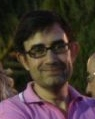
\includegraphics[width = 27mm]{JJM.jpg},] 
\noindent\emph{JJ Merelo} es catedr\'{a}tico de Universidad
en el \'area de Arquitectura y Tecnolog\'{\i}a de Computadores, y
actualmente director de la Oficina de Software Libre de la UGR.
Mantiene un blog desde el a\~no 2002, y lo ha utilizado en clase desde
el a\~no 2004; tambi\'en wikis, agregadores y repositorios de c\'odigo
como herramientas docente. \'{U}ltimamente le ha dado por el \textsl{flipped
learning}, de lo que se informar\'{a} debidamente en esta columna.
\end{window}}}

\medskip

{\small{\begin{window}[0,r,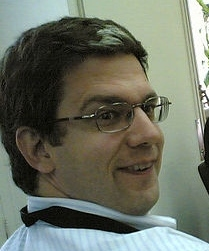
\includegraphics[width = 27 mm]{FTricas1.jpg},]
		\noindent \emph{Fernando Tricas Garc\'{\i}a} es profesor
		titular de Lenguajes y Sistemas Inform\'{a}ticos del Departamento
		de Inform\'{a}tica e Ingenier\'{\i}a de Sistemas de la Universidad de
		Zaragoza.  Empez\'{o} a estudiar la blogosfera casi cuando a\'{u}n no
		exist\'{\i}a (all\'{a} por el a\~{n}o 2002) y a tratar de integrarla en los
		cursos y tareas docentes un poco despu\'{e}s.  Ha impartido
		numerosas charlas relacionadas con el tema de la Web 2.0, 
		internet y universidad,\ldots\ 
		Es actualmente Vicerrector de Tecnolog\'{\i}as de la Informaci\'{o}n y
de la Comunicaci\'{o}n.   
		\end{window}}}
%-------------------------------------------------

		



\noindent 
\bigskip

\noindent\emph{Todas las columnas de la serie Docencia 2.0
pueden descargarse en formato LaTeX desde
\surl{https://github.com/ReVision-Docencia-20/Columnas}}

\noindent\rule{90mm}{1pt}

{\small \noindent\copyright 2016 JJ. Merelo, F. Tricas. Este art\'{\i}culo es de acceso libre distribuido bajo los t\'{e}rminos
de la Licencia Creative Commons de Atribuci\'{o}n, que permite copiar,
distribuir y comunicar p\'{u}blicamente la obra en cualquier medio, s\'{o}lido
o electr\'{o}nico, siempre que se acrediten a los autores y fuentes
originales}

\end{multicols}
\end{document}
